\documentclass[12pt]{article}\usepackage[]{graphicx}\usepackage[]{color}
%% maxwidth is the original width if it is less than linewidth
%% otherwise use linewidth (to make sure the graphics do not exceed the margin)
\makeatletter
\def\maxwidth{ %
  \ifdim\Gin@nat@width>\linewidth
    \linewidth
  \else
    \Gin@nat@width
  \fi
}
\makeatother

\definecolor{fgcolor}{rgb}{0.345, 0.345, 0.345}
\newcommand{\hlnum}[1]{\textcolor[rgb]{0.686,0.059,0.569}{#1}}%
\newcommand{\hlstr}[1]{\textcolor[rgb]{0.192,0.494,0.8}{#1}}%
\newcommand{\hlcom}[1]{\textcolor[rgb]{0.678,0.584,0.686}{\textit{#1}}}%
\newcommand{\hlopt}[1]{\textcolor[rgb]{0,0,0}{#1}}%
\newcommand{\hlstd}[1]{\textcolor[rgb]{0.345,0.345,0.345}{#1}}%
\newcommand{\hlkwa}[1]{\textcolor[rgb]{0.161,0.373,0.58}{\textbf{#1}}}%
\newcommand{\hlkwb}[1]{\textcolor[rgb]{0.69,0.353,0.396}{#1}}%
\newcommand{\hlkwc}[1]{\textcolor[rgb]{0.333,0.667,0.333}{#1}}%
\newcommand{\hlkwd}[1]{\textcolor[rgb]{0.737,0.353,0.396}{\textbf{#1}}}%
\let\hlipl\hlkwb

\usepackage{framed}
\makeatletter
\newenvironment{kframe}{%
 \def\at@end@of@kframe{}%
 \ifinner\ifhmode%
  \def\at@end@of@kframe{\end{minipage}}%
  \begin{minipage}{\columnwidth}%
 \fi\fi%
 \def\FrameCommand##1{\hskip\@totalleftmargin \hskip-\fboxsep
 \colorbox{shadecolor}{##1}\hskip-\fboxsep
     % There is no \\@totalrightmargin, so:
     \hskip-\linewidth \hskip-\@totalleftmargin \hskip\columnwidth}%
 \MakeFramed {\advance\hsize-\width
   \@totalleftmargin\z@ \linewidth\hsize
   \@setminipage}}%
 {\par\unskip\endMakeFramed%
 \at@end@of@kframe}
\makeatother

\definecolor{shadecolor}{rgb}{.97, .97, .97}
\definecolor{messagecolor}{rgb}{0, 0, 0}
\definecolor{warningcolor}{rgb}{1, 0, 1}
\definecolor{errorcolor}{rgb}{1, 0, 0}
\newenvironment{knitrout}{}{} % an empty environment to be redefined in TeX

\usepackage{alltt}
\usepackage[english]{babel}
\usepackage[utf8]{inputenc}
\usepackage{amsmath}
\usepackage{graphicx}
\usepackage{cite}
\usepackage{url}
\usepackage{caption}
\usepackage{setspace}
\IfFileExists{upquote.sty}{\usepackage{upquote}}{}
\usepackage{listings}
\lstset{
	language=R,
	basicstyle=\ttfamily
}

\begin{document}

\begin{titlepage}

\newcommand{\HRule}{\rule{\linewidth}{0.5mm}} % Defines a new command for the horizontal lines, change thickness here

\center % Center everything on the page
 
%----------------------------------------------------------------------------------------
%   HEADING SECTIONS
%----------------------------------------------------------------------------------------

\textsc{\LARGE Montana State University}\\[1.5cm] % Name of your university/college
\textsc{\Large Department of Mathematical Sciences}\\[0.5cm] % Major heading such as course name
\textsc{\large Writing Project}\\[0.5cm] % Minor heading such as course title

%----------------------------------------------------------------------------------------
%   TITLE SECTION
%----------------------------------------------------------------------------------------

\HRule \\[0.4cm]
{ \huge \bfseries Investigation of ESPN's Total Quaterback Rating}\\[0.4cm] % Title of your document
\HRule \\[1.5cm]
 
%----------------------------------------------------------------------------------------
%   AUTHOR SECTION
%----------------------------------------------------------------------------------------

\begin{minipage}{0.4\textwidth}
\begin{flushleft} \large
\emph{Author:}\\
Justin \textsc{Gomez} % Your name
\end{flushleft}
\end{minipage}
~
\begin{minipage}{0.4\textwidth}
\begin{flushright} \large
\emph{Supervisor:} \\
Dr. Mark \textsc{Greenwood} % Supervisor's Name
\end{flushright}
\end{minipage}\\[2cm]

%----------------------------------------------------------------------------------------
%   DATE SECTION
%----------------------------------------------------------------------------------------

{\large May 5, 2017}\\[2cm] % Date, change the \today to a set date if you want to be precise

%----------------------------------------------------------------------------------------
%   LOGO SECTION
%----------------------------------------------------------------------------------------


\includegraphics[width=5cm]{MSU-vert.png} % Include a department/university logo - this will require the graphicx package
 
%----------------------------------------------------------------------------------------

A writing project submitted in partial fulfillment\\
of the requirements for the degree\\[.25in]

\vfill % Fill the rest of the page with whitespace

\end{titlepage}

\begin{titlepage}
\null
\vspace{1.in}
\begin{center}
{\bf\huge APPROVAL}\\[1.in]
of a writing project submitted by\\[.25in]
Justin Gomez \\[1.in]
\end{center}
\noindent
This writing project has been read by the writing project advisor and
has been found to be satisfactory regarding content, English usage,
format, citations, bibliographic style, and consistency, and is ready
for submission to the Statistics Faculty.

\vspace{.3in}
\begin{center}
\begin{tabular}{ll}
\rule{2.75in}{.03in} & \rule{2.75in}{.03in} \\
Date& Mark C. Greenwood \\
& Writing Project Advisor \\
\end{tabular}
\end{center}

\vspace{1cm}

\begin{center}
\begin{tabular}{ll}
\rule{2.75in}{.03in} & \rule{2.75in}{.03in} \\
Date& Mark C. Greenwood \\
& Writing Projects Coordinator \\
\end{tabular}
\end{center}

\end{titlepage}

\newpage
\tableofcontents
\newpage

\begin{abstract}
In 2011, ESPN developed a metric, total quarterback rating (QBR), to project all the aspects of a quarterback's game performance into a single performance index. This statistic is reportedly difficult to calculate, taking thousands of lines of complicated code that supposedly includes situational adjustments to weight various positive or negative components of a quarterback’s performance, although ESPN has never been specific about what is going on in these thousands of lines of code. This fairly vague explanation leaves many wondering how their statistic is actually calculated. In an attempt to answer this question, we will look at four methods to build models that predict QBR using end of game summary information that is easily obtained from the “box score”. In order of simplicity, we will fit linear models, generalized additive models, regression trees, and finally random forests. In addition to these methods, we will look at two algorithms intended to improve predictive accuracy: bagging and boosting. Several sets of predictor variables will be defined and utilized by the appropriate methods, refining models as appropriate to each method. To analyze the predictive accuracy of each model, the data was split into three sets: a training set to build the models, a testing set to assess predictive power, and a validation set to be used only once on the final chosen model. Root mean squared error can be calculated for each model using the testing set, and this metric can be compared across model and methods to select the best predictive model. After fitting six models with various combinations of predictors to our four methods and utilizing our improvement algorithms, it appears as though accurately predicting total quarterback rating is beyond the ability of our specified methods.
\end{abstract}

\doublespacing

\section{Introduction}

In American football, the success of a team can often be attributed to two things: the quarterback and the defense. A team without at least either a great quarterback or a solid defense cannot win often, and they definitely cannot make their way to the Super Bowl to compete for the sport's biggest title. If we take a closer look at these two keys to success we will notice a huge difference other than the side of the ball they play on. The defense is a team of about twenty-six players on the fifty-three man roster, with around twenty-two dressing out for any given game \cite{anat}. That's a lot of players working together to stop an offense, and while a defense's success can be boiled down to a few key players, it takes everyone doing their job to be successful play after play. Even the top defensive players may not be very involved in some plays and may be substituted in and out of play. On the other side, however, is the quarterback, who touches the ball on nearly every play. Just a single person, coordinating the offense on the field, often determining which play is run, and doing his best to lead his team to victory. While there are also about twenty-one \cite{anat} other offensive players on the active game day roster, and their contributions are important, a team cannot move the football down the field and score without a good leader. The quarterback is responsible for so much in a game: communicating plays to teammates, reading the defense, re-positioning offensive players, watching the play clock, handling the snap, and executing the play. And those are just the basics. Quarterbacks have become so valuable to teams, that not only have their salaries seen a great bump as the passing game became more prominent, but so have the salaries of those that are tasked with protecting the quarterback and those that are trying to get to him. Figure~\ref{fig:sal} shows average salaries for current players (2016-2017) in the NFL by position.

\begin{figure}[h]
\centering
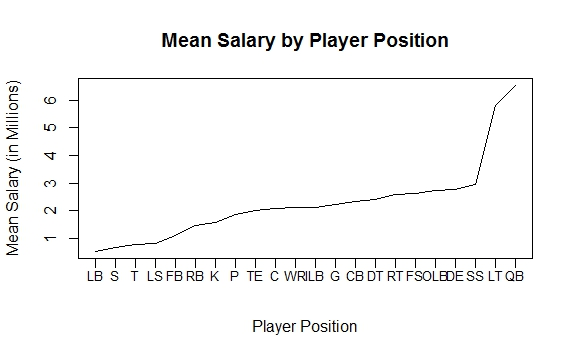
\includegraphics[width=1.2\textwidth]{salary.jpeg}
\captionsetup{font=footnotesize,labelfont=footnotesize}
\caption{\label{fig:sal} Average salary for current (2016-2017) NFL players by position. Data acquired from www.spotrac.com/nfl/contracts/.}
\end{figure}

\newpage
We can see that quarterbacks (QB in the plot) are paid head and shoulders above most of the league. The next highest mean salary is the left tackle (LT). This player is responsible for protecting the quarterback, typically more so than the right tackle (RT) or any other lineman (LB and ILB). Good left tackles keep quarterbacks from taking heavy hits, and are thus valued highly. The final feature to point out in this plot is the average salary of defensive ends (DE), fourth on the list. These players are the ones responsible for putting the pressure on quarterbacks, and disrupting a quarterback's game often results in a loss for that quarterback. 

With so much of the game and its mechanics revolving around this one player, it makes sense that analysts would be interested in a summary measure that would convey how well a quarterback performed during the game. The NFL has its own measure called ``passer rating", which ranges from 0 to 158.3. For a long time this was the measure that was used to compare quarterbacks. However, there are several drawbacks to this statistic. While the NFL clearly defines how their measure is calculated \cite{passer}, the scale is somewhat difficult to interpret as it is not a natural range of values and it is unclear exactly what a one point difference means. Perhaps the biggest drawback however, comes from the measure's purpose. Passer rating is only meant to describe how well a quarterback passed in a game, and it leaves out all of the other things that the quarterback does in any given play. Passer rating uses only completion percentage, average yards gained per pass attempt, percentage of touchdown passes per pass attempt, and percentage of interceptions per pass attempt, all of which are important, but we are still missing some important information such as rushing yards and touchdowns, both of which are much more common to see from today's quarterbacks. The ``dual-threat" quarterback as they are referred to today is seeing increase in value as they can escape intense pass-rushing defenses and extend the play in a multitude of ways. In an attempt to improve upon the NFL's passer rating, ESPN developed their own statistic: total quarterback rating (total QBR or, simply QBR). This measure is much more complicated, and involves taking a closer look at each play the quarterback is involved in.

\subsection{Total Quarterback Rating}
Let's take a look at how EPSN's QBR tries to better capture the performance of a quarterback. Along with outcomes of each play, their model has four major components: win probability, expected points, division of credit, and a ``clutch" index. The win probability comes from a complex analysis of hundreds of past games which were used to develop a win probability function that accounts for a myriad of factors such as field position, time left on the game clock, down, whether a team has home field advantage, etc. Expected points then look at how many points the quarterback's team is expected to gain on any given drive. A drive starting from your own ten yard line is expected to gain fewer points than a drive starting from the opponent's forty yard line. This is where the performance of the quarterback, in terms of passing yards, rushing yards, etc., comes into the model. However, ESPN realizes that the result of every play is not solely because of the quarterback, and so they also build a division of credit aspect into their model. This aspect accounts for the plays where the quarterback makes a lousy throw and the receiver is forced to make a great catch to extend the play. This also accounts for the quarterback making an excellent throw and the receiver dropping the ball. The final piece of the model, the ``clutch" index, analyzes each play and determines how important that play was to the outcome of the game. Throwing for a first down on a fourth down with ten yards to go in the final minutes of a tied game will have a higher rating on the clutch index than a similar play when the score is thirty-five to three. All of these pieces combined, and scaled to be between zero and one hundred, yield the total quarterback rating. According to Dean Oliver from ESPN, calculating this summary statistic requires thousands of lines of code \cite{qbr1}, and given all of the factors that are taken into account play-by-play, one can see why. But is all of this work truly necessary? Can we reconstruct the same total quarterback ratings based on a set of post-game measurements, avoiding the need to process every play of the game?

\subsection{Study Design}
To answer this question, we need as much data on the quarterback as we can collect. Matching the amount of information that goes into QBR will be nearly impossible as much of that data is not made publicly available, but we can still collect the important information that helps summarize how well a quarterback performed. When ESPN introduced QBR in 2011, they went ahead and calculated QBR for quarterbacks all the way back to the 2006 season. We can use information on all the quarterbacks that played for at least twenty action plays (the minimum requirement for QBR to have been calculated) in the last eleven seasons (2006-2016).

Our data comes from two sources: ESPN.com and NFL.com. Total quarterback rating has to be taken from ESPN as it is proprietary, but NFL.com organizes their information in a much more user friendly way, so we will gather all player measures from their site. In our data set we have the following game statistics: number of pass completions, number of pass attempts, total yards gained both passing and rushing, total number of touchdowns scored (again, passing and rushing), number of interceptions thrown, number of sacks taken, number of fumbles by the quarterback, and the end result of the game (win, loss, tie). Once all of the data have been collected, we end up with n=5058 games to work with (after dropping 252 that had incomplete data, which did not appear to be systematic). Our goal here is prediction: we want to predict total QBR with the end of game data we collected. 

Anytime predictive models are built, we would like to know how well they perform. To obtain this measure, we will split our data into three pieces: a ``training" set that will be used to build our models and will account for about 50\% of our full data set, a ``testing" set that will be used to assess the predictive ability of our models and will account for about 30\% of our full data set, and finally a ``validation" set that will be used only once on the model we choose as our best model. This will provide a final independent score for model performance based on the remaining 20\% of our full data set. The testing data set will be used to tune our models, so it will potentially be tested on several times for each approach we take. Once the best model is selected, the validation set will be used once, and will tell us how well our tuned model performs; no further tuning will be done. To obtain the training data set, we took a stratified random sample of two hundred and thirty-nine games from each season to control for any changes that may have been made to the QBR formula, or to game styles and rules, over time. To create the testing set, we took the remaining data and obtain a stratified random sample of one hundred and forty-three games from each season. The remaining data are the validation set. To develop our predictions, we will look at four methods: linear models, generalized additive models, regression trees, and random forests. Overall performance will be assessed with root-mean squared error, or RMSE,

\begin{equation*}
RMSE=\sqrt{\frac{\sum_{i=1}^n(\hat{y_{i}}-y_{i})^{2}}{n}}.
\end{equation*}

\noindent
This estimates the root-mean squared prediction error when used with a model trained on one data set and making predictions on another \cite{gam}.

\section{Methods}
Before we start fitting models, we should make sure we have an understanding of the four methods we will be using. Knowing how these methods work provides insight into the motivation behind using each and what we hope to accomplish with each method. We will also discuss some ways to improve upon the base model fits for some of these methods. Figure~\ref{fig:flexinterp} displays the methods that we will be utilizing.

\begin{figure}[h]
	\centering
	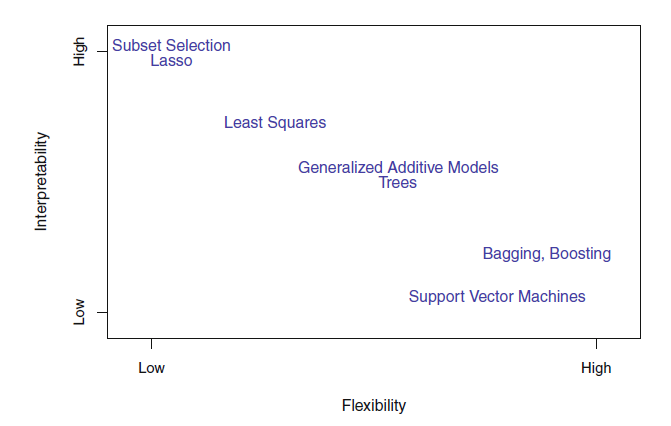
\includegraphics[width=\textwidth]{flexinterp.png}
	\captionsetup{font=footnotesize,labelfont=footnotesize}
	\caption{\label{fig:flexinterp} Plot of model flexibility by model interpretability from \textit{An Introduction to Statistical Learning} \cite{gam}.}
\end{figure}

\newpage
This plot shows an inverse relationship between flexibility and interpretability: as flexibility increases, interpretability decreases. In order of decreasing interpretability, the methods that we will be using are least squares regression (just least squares in the figure), generalized additive models, regression trees, (just trees in the figure), bagging, and boosting. The reverse order then is the order of decreasing flexibility.

\subsection{Linear Models}
Linear models are the simplest, most constrained, and most easily interpreted of the models considered because they only allow for a linear relationship between our explanatory variables and our response variable. Linear models are more commonly used for inference; we can learn a great deal about how our collected data play into determining total QBR by fitting an optimal linear model here. We can learn about ESPN's algorithm if we are able to successfully fit a linear model that generates accurate predictions.

\subsubsection{Explanation}
Perhaps the most commonly used statistical tool, the linear model can be used in a variety of situations and is often a great starting point for any analysis. We use multiple linear regression to estimate our linear models as we have a single quantitative response variable and a suite of predictor variables. For now, we discuss this method in general terms. These models can be written as

\begin{equation} \label{eq:lm}
\boldsymbol{Y}=\boldsymbol{X\beta}+\boldsymbol{\epsilon}.
\end{equation}

In this equation, $\boldsymbol{Y}$ is the vector of responses and $\boldsymbol{X}$ is the matrix of the intercept and the explanatory variables, $x_{1},...,x_{p}$, and each row in the vector or matrix represents the measurements taken on a single observation. $\boldsymbol{\beta}$ is the set of parameters to be estimated for each predictor and $\boldsymbol{\epsilon}$ is the vector of random errors. It is important to note that these models are linear in the $\beta$'s. This distinction allows for a variety of nonlinear transformations to be applied to the set of predictors if necessary to linearize the relationship between \textbf{Y} and the function of $x_{i}$. From this equation, we can see that the goal of these linear models is to estimate $\boldsymbol{\beta}$ so that $\boldsymbol{X\beta}$ is as close to $\boldsymbol{Y}$ as possible, and the difference between $\boldsymbol{X\beta}$ and $\boldsymbol{Y}$ is called the error, or the residuals. 

To generate estimates for $\boldsymbol{\beta}$, we find the values that minimize the sum of the squared residuals, called the least squares estimate, $\boldsymbol{\hat{\beta}}$. This estimate is the best choice provided that  all the assumptions of the Gauss-Markov theorem are met \cite{lm}. The errors need to have a mean of zero with constant variance $\sigma^{2}$, and they also cannot be correlated. As mentioned previously, we also need linearity in our $\beta$ estimates. To generate estimates, $\boldsymbol{X}$ must be full column rank. A normal distribution of the errors is often assumed for inferential purposes, but it is not necessary. Provided these assumptions are all met, then our estimates are the best linear unbiased estimates (commonly referred to as BLUE). Equation~\ref{eq:beta} can be used to generate these values,

\begin{equation} \label{eq:beta}
\boldsymbol{\hat{\beta}}=(\boldsymbol{X}^{T}\boldsymbol{X})^{-1}\boldsymbol{X}^{T}\boldsymbol{y}.
\end{equation}

If we have the correct combination of predictors and our data are representative of the population we are interested in, then our model should generate good predictions for future observations \cite{lm}. But sometimes the true relationships between our predictors and the response is more complicated than a simple additive linear model can explain. So we should also consider interaction terms. These terms allow for the relationship between a predictor variable and the response variable to change as the values of a second predictor variable change. Put another way, the relationship between these variables and the response is not additive. These models can greatly improve fit in many cases and answer more complex questions of interest, and thus several of them will be considered along with several additive models.

\subsection{Generalized Additive Models}
While the assumption of linearity used in multiple regression is often reasonable, sometimes we know that the data we are analyzing do not reasonably meet this assumption, and we would like to use methods that allow for nonlinear relationships to be modeled. Generalized additive models allow for this assumption to be relaxed \cite{gam}. Referring back to Figure~\ref{fig:flexinterp}, recall that these models are more flexible than least squares regression models, and still allow for relatively simple interpretations as the terms are additive.

\subsubsection{Explanation}
Generalized additive models (or GAMs) allow for the addition of nonlinear relationships in such a way that maintains additivity, as the name suggests. Rather than estimating our $\beta$'s as before, we will fit a smooth, nonlinear function for each predictor in our model. Our updated model equation is

\begin{equation} \label{eq:gam}
y_{i}=\beta_{0}+\sum_{i=1}^{p} f_{j}(x_{ij})+\epsilon,
\end{equation}

\noindent
where $f_{j}(x_{ij})$ is a smooth, nonlinear function.

Each of these functions is a smoothing spline, which is a curve generated by a product of estimated coefficients and a chosen set of basis functions, often estimated using penalization to provide simpler estimates.The important thing to note about these splines is that we have the ability to choose the degree of the basis system based on features of our data, and also choose the optimal degree of smoothness exhibited by our spline. GAMs are relatively flexible models that allow us to quickly fit nonlinear relationships in an additive way, and they can often generate more accurate estimates than linear models. Using GAMs here allowed for an assessment of whether the linearity assumption in the linear models was compromising predictive performance. The \texttt{mgcv} \cite{mgcv} package's \texttt{gam} function is used with thin plate splines with shrinkage to estimate a GAM model here.


\subsection{Regression Trees}
Continuing the trend of increasing the potential predictive power of our methods, but losing simple interpretability, we move onto the more sophisticated method of classification trees or regression trees. These are a newer and very powerful method that can produce excellent predictions. In the statistical software R (R Core Team, 2017), there are several packages that fit regression trees. We used \texttt{rpart} \cite{rpart}.

\subsubsection{Explanation}
There are two types of trees that can be used to model a process: classification trees or regression trees. Classification trees are reserved for categorical response variables and regression trees are for quantitative response variables; we built regression trees in our analysis because of the quantitative QBR measure. The primary goal of a tree is partitioning the data set up into uniform sets on the response variable, or at least as uniform as possible. The standard impurity measure for regression trees is $\sum(y_{i}-\bar{y})^{2}$, which is the variation around the mean for each node of the tree.

Splitting is done by looking at the data as a whole, and deciding which variable should be split on first, and where that split should be made. Observations within each subset have similar values of the response. Each subset is then examined, and a variable is again chosen to be split on, making these subsets even more similar on the response variable. This splitting process is repeated recursively until making further splits will no longer greatly improve the uniformity of the subgroups or no more observations remain to be split. Terminal subgroups, the ones on which further splits are no longer made, are called leaves. Predictions are then generated for each leaf in the tree. This process generates a kind of flow chart, or ``decision tree," sorting current or future observations into subgroups and giving an estimated or predicted total quarterback rating to these observations \cite{gam}. Figure~\ref{fig:part} and Figure~\ref{fig:ex} give an example of a partitioned predictor space, as well as the resulting regression tree for a simple model with completion percentage and number of touchdowns as the predictors of QBR.
\newpage

\begin{figure}[h]
\centering
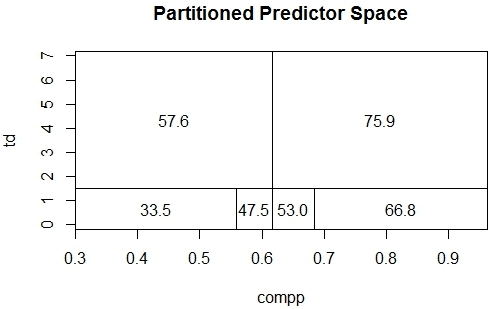
\includegraphics[width=.6\textwidth]{expartspace.jpeg}
\captionsetup{font=footnotesize,labelfont=footnotesize}
\caption{\label{fig:part} Example of a partitioned predictor space with explanatory variables completion percentage and touchdowns on the response variable QBR. Partitions, or splits, are shown as solid lines, with the predicted QBR for each partition is shown inside the regions.}
\end{figure}

\begin{figure}[h]
\centering
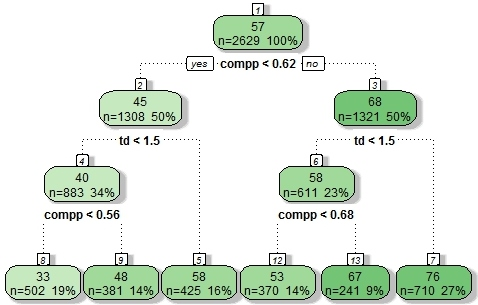
\includegraphics[width=.6\textwidth]{extree.jpeg}
\captionsetup{font=footnotesize,labelfont=footnotesize}
\caption{\label{fig:ex} Resulting regression tree from the previously pictured partitioning. The terminal nodes display the mean, number of observations, and percentage of the data set in that node.}
\end{figure}

\newpage
After a tree has been fully grown, we need to assess whether it is adequate as is or if it is over-fitting the data. Tree growing algorithms are typically ``greedy" and thus often grow too large. The process of only keeping the ``useful" part of the tree is referred to as ``pruning." We start by finding all possible nested trees (trees which contain a subset of splits as the final tree; these are always smaller as we start by removing splits lower down on the tree first). For each nested tree, we assess the degree to which our predictions are improved by, looking for enough improvement to justify making the split. The parameter used to assess this is called the cost-complexity parameter which is chosen to minimize the cross-validated prediction error. Pruning ensures that our predictions are as good as they can be for the given predictor set, but that our trees are not unnecessarily complex.

\subsection{Random Forests}
The final base method we will consider is the most flexible one of the four and naturally builds off of regression trees. Random forests are commonly turned to for quick and reliable predictions and are often regarded as the golden standard of prediction. They are also so complex that interpretations of the underlying mechanics of the forests are difficult to develop. In R, the package \texttt{randomForest} was used \cite{randomForest}.

\subsubsection{Explanation}
Random forests are exactly what they sound like: a random collection of fitted trees combined to generate predictions. If we fit trees according to our previously outlined methods, we'll end up with the same tree, over and over, which is not useful. That's where randomness comes in. Random forests have the advantage of generating many trees that differ from each other, resulting in less variable and thus more powerful predictions once they are aggregated. Normally, we consider all the variables when making a split and choose the best one, and if there is an especially useful explanatory variable, this will usually be the one the split is made on. This is what leads to relatively little difference in fitted trees, even if we used different subsets of the data. Random forests however only consider a random sample of predictors at each split, typically the number of parameters divided by three (rounded down if necessary). 

Another random component of this method also exists in the data used to grow each tree. Rather than using the full training data set, a bootstrap sample is obtained and the tree is grown on this bootstrap sample. A bootstrap sample is a sample of the same size as the original, and is obtained by sampling observations from the original sample with replacement. This generates a sample that may contain the same observation several times and others not at all (on average about 2/3 of the observations in the original sample are selected). This yields many different looking trees, and when we average over all of them we see a large reduction in the variance of our predictions \cite{gam}. For our purposes, a hundred trees are all that are necessary to build our random forests.

\subsection{Improving Predictions}
Now that we have reviewed the primary methods we will be using to fit models, let's discuss a few methods for improving our predictions.

\subsubsection{Bagging}
Linear models on their own do not always have the best predictive ability. One method to help increase a model's predictive ability is Bootstrap AGGregation, or bagging. Bagging is a great way to reduce the variance of the predictions that we obtain from our models, thus giving more stable predicted values. To apply this method on our models, we first must obtain a bootstrap sample of our training data. The desired model is then fit on the bootstrapped data and predictions are obtained like normal. This process of bootstrapping, fitting a model, and obtaining predictions is repeated as many times as desired, usually a large number, and for our study, we will use one thousand iterations. After the thousand sets of predictions are obtained, we aggregate them to obtain a single set of predictions, which can be performed by simply averaging the predictions together. Then, RMSE can be found for this aggregate set of predictions. It should be noted that bagging is not always going to improve a model's prediction accuracy, especially for linear models and GAMs as they are already have relatively low variance \cite{bag}. This algorithm should yield slightly more improvement for trees, however, as the trees resulting from bagging are not pruned and have an increased variance \cite{gam}.

\subsubsection{Boosting}
Bagging can be a useful tool when used in conjunction with trees, but there are other tools that can prove more useful. Where bagging is performed as an independent process (one fitted tree does not depend on the results of any other fitted tree), boosting is a dependent process in that the models are fit sequentially, and the resulting fit from one depends directly on the fit from the tree that came before it. To start, we fit a tree like we would normally using the full training set. Then, we obtain the residuals from the model, and fit a tree on these residuals. We continue on in this fashion, slowly growing trees and improving our model's prediction power. These models are called gradient boosting machines and are available in the \texttt{gbm} package in R \cite{gbm}.

When fitting these boosted models, there are three things to choose: the number of trees to grow, the shrinkage parameter, and the maximum depth of the tree. The number of trees that we want to grow in our boosting procedure is important as we do not want to cut off the learning procedure too early and end up with a partially boosted model that might not fit as well as it could. The shrinkage parameter helps control how quickly, or slowly, the models learn. Typically, we want the models in this method to grow slowly to avoid over-fitting, so shrinkage parameters of 0.01 or 0.001 are most often used. The last piece to control in this method is the maximum depth of the tree. This translates to the number of splits that we will have in our tree. A large number of splits, or a deep tree, typically leads to over-fitting, so some thought should be given to this parameter selection \cite{bag}. For our study, we will fit one thousand trees with a shrinkage parameter of 0.01, and a maximum depth of two splits.

To understand this method better, let's look at a toy example. Consider sampling fifty points from the function $y=cos(x)$ for $x \in [0,5]$. We want to apply the method of gradient boosting to regression trees to accurately predict this function over the specified interval. Figure~\ref{fig:boostex} shows six trees fitted according to the boosting algorithm, and Figure~\ref{fig:combine} shows the combined predictions compared to the underlying truth and the sampled points.

\begin{figure}[h]
	\centering
	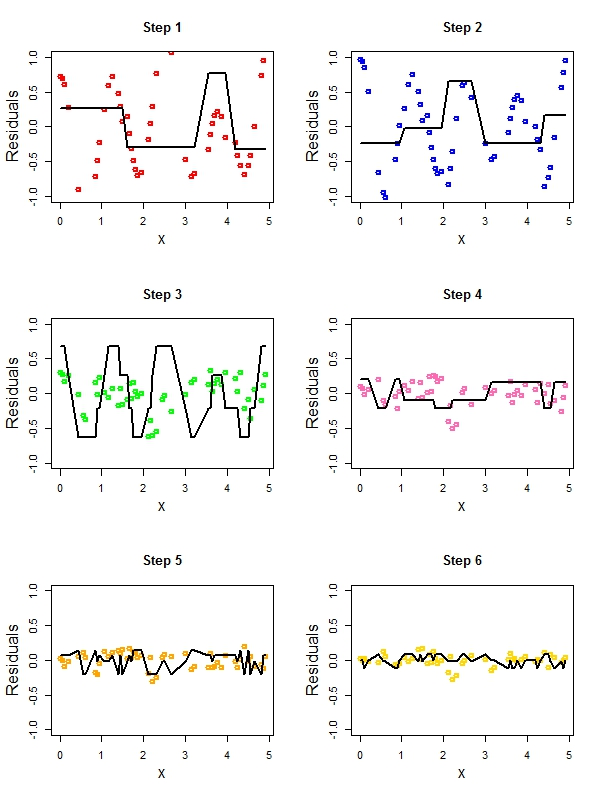
\includegraphics[width=.8\textwidth]{boostex.jpeg}
	\captionsetup{font=footnotesize,labelfont=footnotesize}
	\caption{\label{fig:boostex} Sequentially fit trees according to the boosting algorithm. Each plot shows the predictions as a solid line and the residuals as the scattered dots around the predictions. Note that these trees were grown simply as an example to illustrate a point, and in practice we would likely not need to grow all of these trees. Additionally, the individual trees are more complex than those used for the QBR models.}
\end{figure}

\begin{figure}[h]
	\centering
	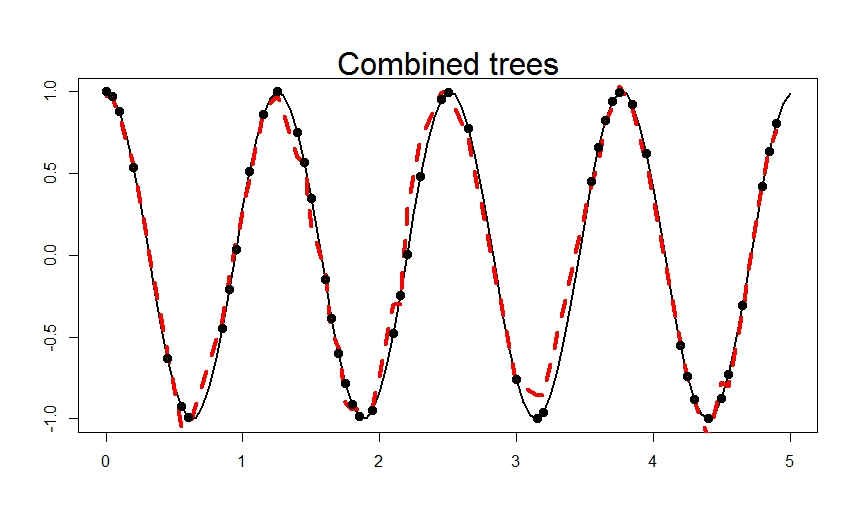
\includegraphics[width=.8\textwidth]{combine.jpeg}
	\captionsetup{font=footnotesize,labelfont=footnotesize}
	\caption{\label{fig:combine} Plot of the underlying truth with the predicted values over the full range overlaid. Originally sampled points are also shown.}
\end{figure}

\newpage
\section{Fitted Models}
Before we begin fitting models according to specific methods, let's discuss the models that we will consider fitting with the different methods. Our data set consists of the eight previously discussed game statistics. To understand the relationships present between the quantitative variables, it may be helpful to examine their correlations provided in Figure~\ref{fig:corr}.

\begin{figure}[h]
\centering
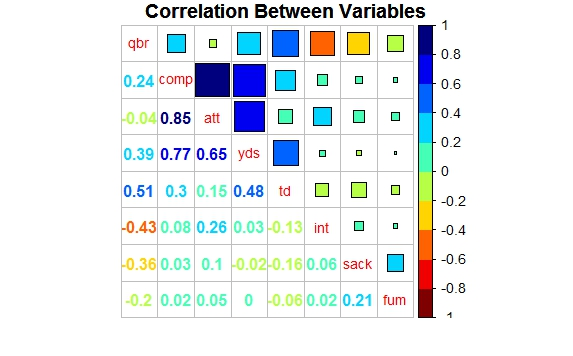
\includegraphics[width=1.2\textwidth]{correlation.jpeg}
\captionsetup{font=footnotesize,labelfont=footnotesize}
\caption{\label{fig:corr} Plot of the correlations between quantitative variables. Size and color of the squares indicate the strength and direction of the relationship. The lower diagonal also gives the correlation coefficients, rounded to two decimal places.}
\end{figure}

Many of the relationships that we see are not surprising, such as the strong positive correlation between the number of completions and the number of attempts, or the number of completions and the number of yards. We can also get a sense for each variable's relationship with QBR by examining the first row and column. Again, not many surprises here. We see positive relationships with completions, yards, and touchdowns, and negative relationships with interceptions, sacks, and fumbles. The only relationship that is a little surprising is the weak negative relationship between pass attempts and QBR, although this may be due to the fact that, in general, quarterbacks in losing situations make more passes. Perhaps a better way to bring passing attempts and completions into the model would be as completion percentage, defined as the number of completions divided by the number of attempts. Figure~\ref{fig:corr2} displays the relationships between the variables with completion percentage rather than the two separate variables, and Figure~\ref{fig:allthescatters} displays plots of each quantitative variable against QBR.

\begin{figure}[h]
\centering
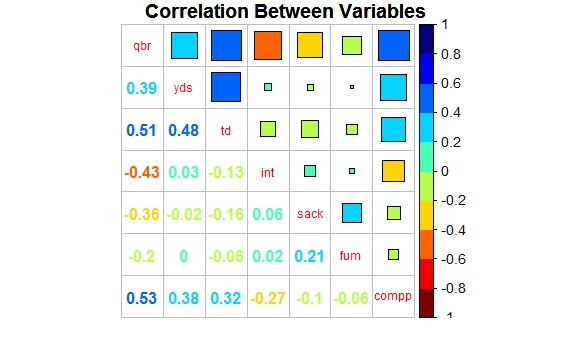
\includegraphics[width=1.2\textwidth]{correlation2.jpeg}
\captionsetup{font=footnotesize,labelfont=footnotesize}
\caption{\label{fig:corr2} Plot of the correlations between quantitative variables with completion percentage rather than number of completions and number of attempts.}
\end{figure}

\begin{figure}[h]
	\centering
	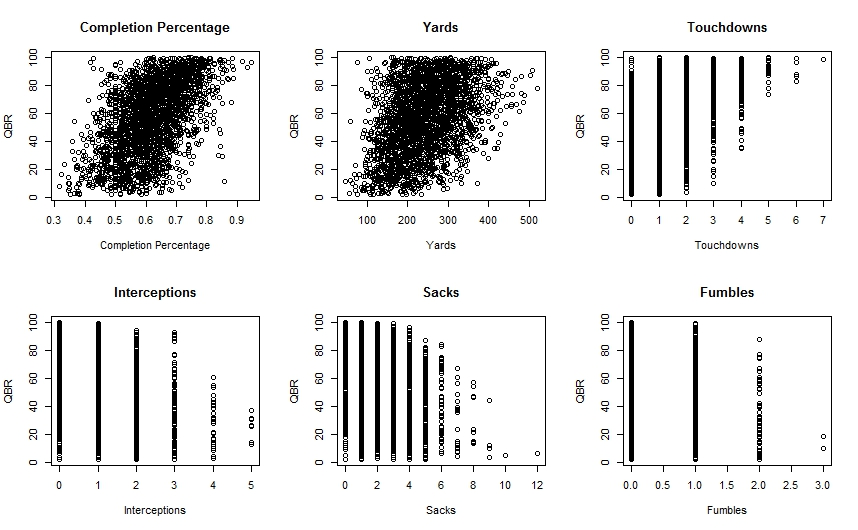
\includegraphics[width=.9\textwidth]{allthescatters.jpeg}
	\captionsetup{font=footnotesize,labelfont=footnotesize}
	\caption{\label{fig:allthescatters} Plots of the quantitative variables against QBR.}
\end{figure}

The relationships between the variables and completion percentage (compp in the figure) are not altogether unexpected. With all of this information, we can build a few candidate models. Naturally, for all these models total QBR is the response variable. We will consider three additive models and three models with interactions. The largest additive model (Model 1) has the six important summary statistics of a quarterbacks performance: completion percentage, total yards, number of touchdowns, number of fumbles, number of interceptions thrown, and number of times sacked, as well as the result of the game (win or loss). The second model (Model 2) has all these variables except for the end result of the game, and the smallest additive model (Model 3) has only four predictors, completion percentage, number of interceptions thrown, number of touchdowns, and total yards. Our interaction models will include all seven predictors as main effects, regardless of the interactions included. The first interaction model (Model 4) will have three pairwise interactions between completion percentage and fumbles, interceptions, and touchdowns. The next model (Model 5) considers three pairwise interactions between the number of sacks and the result of the game, touchdowns, and interceptions. Finally, our third interaction model (Model 6) will include three pairwise interactions between total yards and touchdowns, interceptions, and fumbles. Using these different combinations of variables will act as our tuning step when we begin fitting our models according to the various methods. Table~\ref{tab:models} summarizes the variables that are going into each model.

\begin{table}[h]
\centering
\begin{tabular}{|c|c|c|c|c|c|c|}
\hline
Variables & Model 1 & Model 2 & Model 3 & Model 4 & Model 5 & Model 6\\
\hline
Completion Percent & X & X & X & I & X & X \\
\hline
Yards & X & X & X & X & X & I \\
\hline
Touchdowns & X & X & X & I & I & I \\
\hline
Interceptions & X & X & X & I & I & I \\
\hline
Sacks & X & X &  & X & I & X \\
\hline
Fumbles & X & X &  & I & X & I \\
\hline
Game Result & X & & & X & I & X\\
\hline
\end{tabular}
\captionsetup{font=footnotesize,labelfont=footnotesize}
\caption{\label{tab:models} Table summarizing the variables in each model. `X' indicates the variable is included in that model and `I' indicates the variable is included as part of an interaction term.}
\end{table}

When it comes to fitting these models according to specific methods, we can use Models 1-6 for least squares regression but for generalized additive models, regression trees, and random forests, we will only use Models 1-3 as these methods do not allow for the specification of interactions as we would with linear regression. When we fit the GAMs, we will fit three df thin plate splines with shrinkage as our splines for each variable. When we perform our bagging and boosting algorithms on each method, we will use the same specified models as we did before performing the improvement.

\section{Results}
Now that the methods used have been discussed and the models defined, let's take a look at how well each model performs.

\subsection{Linear Models}
First up are the linear models. Table~\ref{tab:lmres} summarizes the results of the six fitted linear models, along with the bagging results. Many of the values in Table~\ref{tab:lmres} are similar. We can see that bagging the linear models did not show a great decrease in RMSE, but that was to be expected for these models. The poorest performer is also the smallest model in our set with only four predictors (RMSE of 18.150), which is to be expected. From there, most of the other models have RMSEs around 16.1. The best additive model is the largest model with all of our predictors, and the best model with interaction terms is model six with the three pairwise interactions between yards and touchdowns, interceptions, and fumbles. Overall, it does not appear as though a linear model is able to completely predict total QBR.

\begin{table}[h]
\centering
\begin{tabular}{|c|c|c|}
\hline
Model & RMSE & RMSE, Bagged \\
\hline
1 & 16.104 & 16.103 \\
\hline
2 & 16.323 & 16.323 \\
\hline
3 & 18.150 & 18.149 \\
\hline
4 & 16.045 & 16.045 \\
\hline
5 & 16.111 & 16.112 \\
\hline
6 & 15.940 & 15.940 \\
\hline
\end{tabular}
\captionsetup{font=footnotesize,labelfont=footnotesize}
\caption{\label{tab:lmres} Table of RMSE's for fitted linear models and bagged linear models on the testing data set.}
\end{table}

Moving on to our next modeling method, the generalized additive models, we hope to see an improvement, even if only slightly. Table~\ref{tab:gamres} summarizes the results of fitting GAMs to the additive models and bagging these models. We see relatively similar results for these models as we did with the linear models. Interestingly enough, all of the bagged GAMs performed worse than the original models, as indicated by the slightly increased RMSEs, although these aren't extremely large increases on this scale. This could be due to the fact that we are fitting smoothing splines with these models, and when we perform the bagging process, we are only looking at a bootstrap sample of our full training set, meaning there is typically less information to fit our splines with, which affects the overall fit. We also see the same pattern of performance in these models; our smallest model performs the worst, and the fullest model performs the best. Again, these RMSEs are higher than we would like in order to say we can accurately predict total QBR.

\begin{table}[h]
\centering
\begin{tabular}{|c|c|c|}
\hline
Model & RMSE & RMSE, Bagged \\
\hline
1 & 15.963 & 15.974 \\
\hline
2 & 16.160 & 16.175 \\
\hline
3 & 18.005 & 18.040 \\
\hline
\end{tabular}
\captionsetup{font=footnotesize,labelfont=footnotesize}
\caption{\label{tab:gamres} Table of RMSE's for fitted generalized additive models and bagged generalized additive models on the testing data set.}
\end{table} 

Perhaps regression trees will fit better. Table~\ref{tab:treeres} gives the RMSEs for the three pruned trees, as well as the bagged and boosted results. Before discussing what we learn from ~\ref{tab:treeres}, we can plot each tree to get a sense for how each tree is processing the information in our training dataset. Figure~\ref{fig:tree1} displays the tree for the full set of predictors and Figure~\ref{fig:tree2} displays the tree for the two smaller models, which interestingly enough yield the same tree after pruning. Figure~\ref{fig:treecp} display the complexity parameters used to prune each tree.

\begin{table}[h]
\centering
\begin{tabular}{|c|c|c|c|}
\hline
Model & RMSE & RMSE, Bagged & RMSE, Boosted \\
\hline
1 & 20.667 & 18.806 & 16.062\\
\hline
2 & 20.655 & 18.615 & 16.238\\
\hline
3 & 20.655 & 19.203 & 18.102\\
\hline
\end{tabular}
\captionsetup{font=footnotesize,labelfont=footnotesize}
\caption{\label{tab:treeres} Table of RMSE's for pruned trees, as well as their bagged and boosted results.}
\end{table}

\newpage

\begin{figure}[h]
\centering
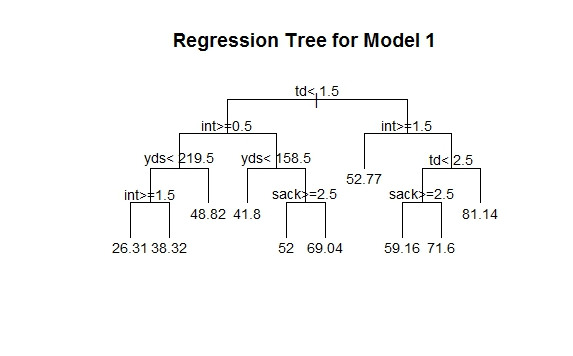
\includegraphics[width=1.1\textwidth]{tree1.jpeg}
\captionsetup{font=footnotesize,labelfont=footnotesize}
\caption{\label{fig:tree1} Regression tree for the full set of predictor variables.}
\end{figure}
\newpage

\begin{figure}[h]
\centering
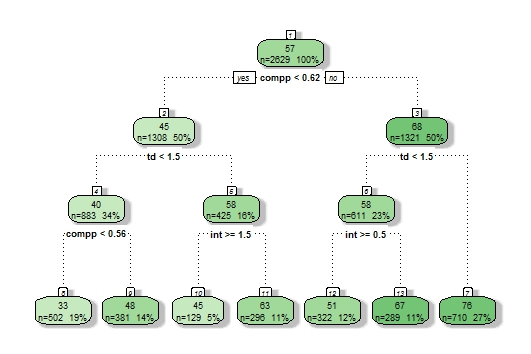
\includegraphics[width=1.1\textwidth]{tree2.jpeg}
\captionsetup{font=footnotesize,labelfont=footnotesize}
\caption{\label{fig:tree2} Regression tree for the middle and smallest sets of predictor variables.}
\end{figure}

\newpage

\begin{figure}[h]
\centering
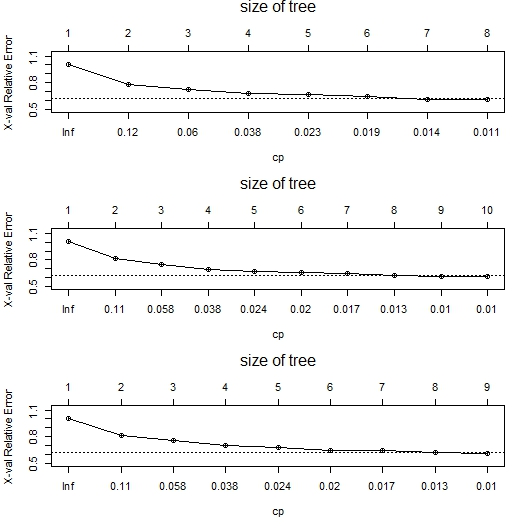
\includegraphics[width=.9\textwidth]{treecp.jpeg}
\captionsetup{font=footnotesize,labelfont=footnotesize}
\caption{\label{fig:treecp} Plots of the complexity parameters for all three sets of predictors. The top plot is for the full set of seven variables and the bottom plot is for the smallest set of variables. The trees are pruned to the simplest tree within one standard error of the minimum cross-validated error.}
\end{figure}

\newpage
It is interesting to see how each tree works with the set of information it's given. For example, the tree built on the full set of variables (Figure~\ref{fig:tree1}) is slightly smaller than the trees built on fewer variables (Figure~\ref{fig:tree2}). It also chooses to make a split on result first, which is one of the variables that the other two did not have available to them. As a binary outcome, it seems to make sense that observations in each category are more similar to each other than they would be to observations in the other category. The percentages in the leaves of each tree tell us the percent of the data that ended up in that node. Thinking back to Table~\ref{tab:treeres}, we see that these simple pruned trees do not predict as well as their linear model counterparts. Even the bagged trees aren't as well at predicting, and it isn't until we perform gradient boosting that the trees start to predict as good as the linear models.

Before reflecting on this, there is one more tool left to generate predictions: the random forest. Table~\ref{tab:forestres} summarizes the results for the models with this method. These results, which were supposed to be the best that we would see, are not any better than our original linear models. That makes three sets of more sophisticated methods (GAMs, trees, forests) and two algorithms for improvement (bagging and boosting) that should have generated better predictions than linear models by themselves, and yet they all failed to. We see relatively high RMSEs across the board, hovering around sixteen for just about every model that we fit with our various methods. Plots of fitted versus residuals plots are provided in Figure~\ref{fig:residbyfit} for the top fitting model in each method.

\begin{table}[h]
\centering
\begin{tabular}{|c|c|}
\hline
Model & RMSE \\
\hline
1 & 16.622\\
\hline
2 & 16.937\\
\hline
3 & 18.419\\
\hline
\end{tabular}
\captionsetup{font=footnotesize,labelfont=footnotesize}
\caption{\label{tab:forestres} Table of RMSE's for the three fitted random forests on the testing data set.}
\end{table}

\begin{figure}[h]
	\centering
	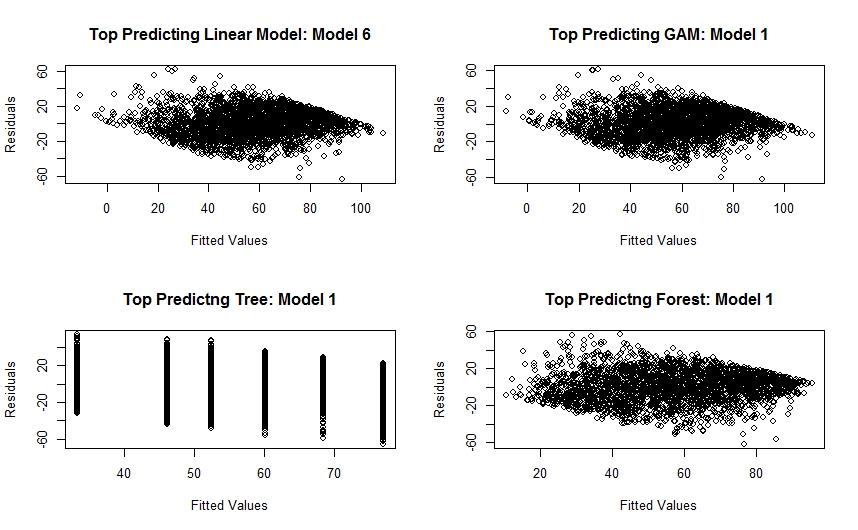
\includegraphics[width=\textwidth]{residbyfit.jpeg}
	\captionsetup{font=footnotesize,labelfont=footnotesize}
	\caption{\label{fig:residbyfit} Fitted versus residuals plots for the four methods.}
\end{figure}

\section{Conclusion}
With all of these fitted models, we still have one task left: we need to pick the best performing model to generate predictions with using our validation set. Recall that this set was set aside before the analysis began and has not been used yet.

\subsection{Final Model Selection}
In the beginning, it was assumed that gradient boosted trees or random forests would come out on top, but the model that produced the smallest root-mean squared error on the testing set is the linear model with pairwise interactions between yards and touchdowns, interceptions, and fumbles. This is the model that we used on our validation set. The fitted model is as follows:

\begin{multline*}
\widehat{QBR}_{i}=-0.765+63.148compp_{i}-7.331fum_{i}-8.446int_{i}-3.432sack_{i}+10.498td_{i}+\\
0.085yds_{i}+2.167result_{Li}+9.240result_{Wi}-0.021td_{i}\times yds_{i}+\\
0.005int_{i}\times yds_{i}+0.010fum_{i}\times yds_{i}.\\
\end{multline*}

Using this model to generate predictions gives us the fitted versus residuals plot in Figure~\ref{fig:finally}.

\begin{figure}[h]
	\centering
	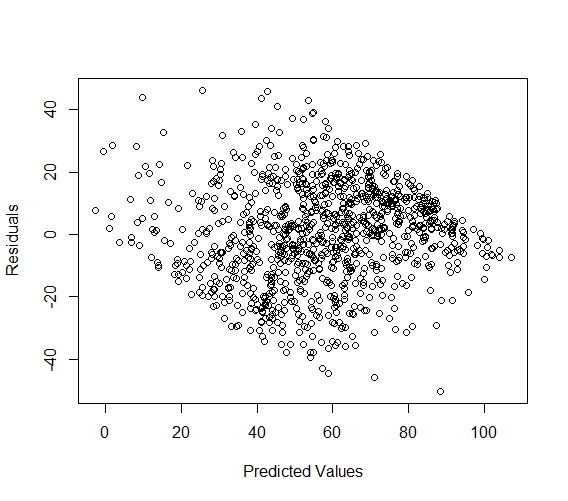
\includegraphics[width=\textwidth]{finally.jpeg}
	\captionsetup{font=footnotesize,labelfont=footnotesize}
	\caption{\label{fig:finally} Fitted versus residuals plots for the final set of predictions with the specified linear model on the validation data set.}
\end{figure}

\noindent
This final set of predictions looks very similar to the other sets that were generated in Figure~\ref{fig:residbyfit}. The RMSE on this validation set is 15.716, which is on par with what we found on the testing set.

\subsection{Final Thoughts}
After fitting a variety of models with a suite of methods, what have we learned? Recall that we initially set out to predict ESPN's total quarterback rating with post game summaries only, rather than the more intense play-by-play information. Using passing completion percentage, number of fumbles, number of interceptions thrown, sacks taken, total number of touchdowns scored both through rushing and passing, total number of yards gained both through rushing and passing, and finally the result of the game (win, loss, tie). In order of increasing model flexibility, we fit linear models, generalized additive models, regression trees, and random forests, with bagging and boosting algorithms to help improve each model fit. A linear model ended up performing the best, which was not what was expected as random forests or gradient boosted regression trees should produce the best predictions. And regardless of method, the root-mean squared errors for the predictions are generally large, with most values around 16 units on the QBR scale, and the smallest at 15.94 units on the QBR scale. Considering QBR only ranges from zero to one hundred, these models are not overly reliable. They may give us a pretty good idea for how a quarterback performed, but they definitely aren't getting at the same information that ESPN is. Whatever it is that ESPN's algorithm is doing with the play-by-play level information is more than our post-game summaries can get at with the model space and methods we worked with. 

There are several ways this study can be improved and extended in the future. The NFL is has started releasing a set of new statistics the public has never had access to such as maximum and average speeds achieved by players, max distance thrown by the quarterback, and even time from the snap to the release of the football. These are all measures that could help improve our model fits. The model space can also be greatly extended through the use of all subset search methods that test all possible combinations of variables. This may have uncovered other useful interactions but it was not employed here. It would also be interesting to look more specifically into total QBRs for specific players or teams, or even try modeling a player's rating over the course of the season or his career. Perhaps further analysis will uncover even more interesting relationships and allow fans to gain a peak inside this great sport.

\nocite{*}

\newpage
\section{References}
\begin{flushleft}
\bibliographystyle{acm}
\bibliography{wp}
\end{flushleft}

\newpage
\section{Appendix-R Code}
\singlespacing
\begin{lstlisting}
library(corrplot)
library(randomForest)
library(rpart)
library(car)
library(mgcv)
library(gbm)
library(rattle)
library(MuMIn)
library(caret)
library(beanplot)
#read in train and test
train<-read.csv("trainingdata.csv")[,-c(1,15)]
train$compp<-train$comp/train$att
train$result<-factor(train$result,levels=c("T","L","W"))

test<-read.csv("testingdata.csv")[,-c(1,15)]
test$compp<-test$comp/test$att
test$result<-factor(test$result,levels=c("T","L","W"))

#models
mod1<-qbr~compp+fum+int+sack+td+yds+result
mod2<-qbr~compp+fum+int+sack+td+yds
mod3<-qbr~compp+int+td+yds
mod4<-qbr~compp+fum+int+sack+td+yds+result+compp:fum+compp:int+compp:td
mod5<-qbr~compp+fum+int+sack+td+yds+result+sack:result+sack:td+sack:int
mod6<-qbr~compp+fum+int+sack+td+yds+result+yds:td+yds:int+yds:fum

#fitted lms
lm1<-lm(mod1,data=train)
lm2<-lm(mod2,data=train)
lm3<-lm(mod3,data=train)
lm4<-lm(mod4,data=train)
lm5<-lm(mod5,data=train)
lm6<-lm(mod6,data=train)
#AIC comparison
aic<-AIC(lm1,lm2,lm3,lm4,lm5,lm6)[,2]
name<-c("Model 1","Model 2","Model 3","Model 4","Model 5","Model 6")
s<-order(aic)
name<-name[s]
m<-min(aic)
del<-round(aic[s]-m,2)
tab.aic<-data.frame(Model=name,AIC=aic,delta=del)

#lm RMSE
rmse<-function(a){
error<-a-test$qbr
sqrt(mean(error^2))
}
lm.rmse1<-rmse(predict(lm1,newdata=test,type="response"))
lm.rmse2<-rmse(predict(lm2,newdata=test,type="response"))
lm.rmse3<-rmse(predict(lm3,newdata=test,type="response"))
lm.rmse4<-rmse(predict(lm4,newdata=test,type="response"))
lm.rmse5<-rmse(predict(lm5,newdata=test,type="response"))
lm.rmse6<-rmse(predict(lm6,newdata=test,type="response"))

#bagged lms
n<-1000
#mod1
boot.pred<-matrix(12,ncol=n,nrow=nrow(test))
set.seed(4141993)
for (i in 1:n) {
these<-sample(rownames(train),nrow(train)-1,replace=TRUE)
boot<-train[c(these,2463),]
boot$result<-factor(boot$result,levels=c("T","L","W"))
lm.boot<-lm(mod1,data=boot)
boot.pred[,i]<-predict(lm.boot,newdata=test,type="response")
}
mean.pred<-rep(12,nrow(test))
for(i in 1:nrow(test)){
mean.pred[i]<-mean(boot.pred[i,])
}
boot.rmse1<-rmse(mean.pred)
#mod2
boot.pred<-matrix(12,ncol=n,nrow=nrow(test))
set.seed(4141994)
for (i in 1:n) {
these<-sample(rownames(train),nrow(train)-1,replace=TRUE)
boot<-train[c(these,2463),]
boot$result<-factor(boot$result,levels=c("T","L","W"))
lm.boot<-lm(mod2,data=boot)
boot.pred[,i]<-predict(lm.boot,newdata=test,type="response")
}
mean.pred<-rep(12,nrow(test))
for(i in 1:nrow(test)){
mean.pred[i]<-mean(boot.pred[i,])
}
boot.rmse2<-rmse(mean.pred)
#mod3
boot.pred<-matrix(12,ncol=n,nrow=nrow(test))
set.seed(4141995)
for (i in 1:n) {
these<-sample(rownames(train),nrow(train)-1,replace=TRUE)
boot<-train[c(these,2463),]
boot$result<-factor(boot$result,levels=c("T","L","W"))
lm.boot<-lm(mod3,data=boot)
boot.pred[,i]<-predict(lm.boot,newdata=test,type="response")
}
mean.pred<-rep(12,nrow(test))
for(i in 1:nrow(test)){
mean.pred[i]<-mean(boot.pred[i,])
}
boot.rmse3<-rmse(mean.pred)
#mod4
boot.pred<-matrix(12,ncol=n,nrow=nrow(test))
set.seed(4141996)
for (i in 1:n) {
these<-sample(rownames(train),nrow(train)-1,replace=TRUE)
boot<-train[c(these,2463),]
boot$result<-factor(boot$result,levels=c("T","L","W"))
lm.boot<-lm(mod4,data=boot)
boot.pred[,i]<-predict(lm.boot,newdata=test,type="response")
}
mean.pred<-rep(12,nrow(test))
for(i in 1:nrow(test)){
mean.pred[i]<-mean(boot.pred[i,])
}
boot.rmse4<-rmse(mean.pred)
#mod5
boot.pred<-matrix(12,ncol=n,nrow=nrow(test))
set.seed(4141997)
for (i in 1:n) {
these<-sample(rownames(train),nrow(train)-1,replace=TRUE)
boot<-train[c(these,2463),]
boot$result<-factor(boot$result,levels=c("T","L","W"))
lm.boot<-lm(mod5,data=boot)
boot.pred[,i]<-predict(lm.boot,newdata=test,type="response")
}
mean.pred<-rep(12,nrow(test))
for(i in 1:nrow(test)){
mean.pred[i]<-mean(boot.pred[i,])
}
boot.rmse5<-rmse(mean.pred)
#mod6
boot.pred<-matrix(12,ncol=n,nrow=nrow(test))
set.seed(4141998)
for (i in 1:n) {
these<-sample(rownames(train),nrow(train)-1,replace=TRUE)
boot<-train[c(these,2463),]
boot$result<-factor(boot$result,levels=c("T","L","W"))
lm.boot<-lm(mod6,data=boot)
boot.pred[,i]<-predict(lm.boot,newdata=test,type="response")
}
mean.pred<-rep(12,nrow(test))
for(i in 1:nrow(test)){
mean.pred[i]<-mean(boot.pred[i,])
}
boot.rmse6<-rmse(mean.pred)

#fitted gams
gam1<-gam(qbr~s(compp,k=3,bs="ts")+s(yds,k=3,bs="ts")+s(td,k=3,bs="ts")+
s(int,k=3,bs="ts")+s(sack,k=3,bs="ts")+fum+result,data=train)
gam2<-gam(qbr~s(compp,k=3,bs="ts")+s(yds,k=3,bs="ts")+s(td,k=3,bs="ts")+
s(int,k=3,bs="ts")+s(sack,k=3,bs="ts")+fum,data=train)
gam3<-gam(qbr~s(compp,k=3,bs="ts")+s(yds,k=3,bs="ts")+s(td,k=3,bs="ts")+
s(int,k=3,bs="ts"),data=train)

#gam rmse
gam.rmse1<-rmse(predict(gam1,newdata=test,type="response"))
gam.rmse2<-rmse(predict(gam2,newdata=test,type="response"))
gam.rmse3<-rmse(predict(gam3,newdata=test,type="response"))

#bagged gam
#gam1
boot.pred<-matrix(12,ncol=n,nrow=nrow(test))
set.seed(4141993)
for (i in 1:n) {
these<-sample(rownames(train),nrow(train)-1,replace=TRUE)
boot<-train[c(these,2463),]
boot$result<-factor(boot$result,levels=c("T","L","W"))
gam.boot<-gam(qbr~s(compp,k=3,bs="ts")+s(yds,k=3,bs="ts")+s(td,k=3,bs="ts")+
s(int,k=3,bs="ts")+s(sack,k=3,bs="ts")+fum+result,data=boot)
boot.pred[,i]<-predict(gam.boot,newdata=test,type="response")
}
mean.pred<-rep(12,nrow(test))
for(i in 1:nrow(test)){
mean.pred[i]<-mean(boot.pred[i,])
}
gam.boot.rmse1<-rmse(mean.pred)
#gam2
boot.pred<-matrix(12,ncol=n,nrow=nrow(test))
set.seed(4141994)
for (i in 1:n) {
these<-sample(rownames(train),nrow(train)-1,replace=TRUE)
boot<-train[c(these,2463),]
boot$result<-factor(boot$result,levels=c("T","L","W"))
gam.boot<-gam(qbr~s(compp,k=3,bs="ts")+s(yds,k=3,bs="ts")+s(td,k=3,bs="ts")+
s(int,k=3,bs="ts")+s(sack,k=3,bs="ts")+fum,data=boot)
boot.pred[,i]<-predict(gam.boot,newdata=test,type="response")
}
mean.pred<-rep(12,nrow(test))
for(i in 1:nrow(test)){
mean.pred[i]<-mean(boot.pred[i,])
}
gam.boot.rmse2<-rmse(mean.pred)
#gam3
boot.pred<-matrix(12,ncol=n,nrow=nrow(test))
set.seed(4141995)
for (i in 1:n) {
these<-sample(rownames(train),nrow(train)-1,replace=TRUE)
boot<-train[c(these,2463),]
boot$result<-factor(boot$result,levels=c("T","L","W"))
gam.boot<-gam(qbr~s(compp,k=3,bs="ts")+s(yds,k=3,bs="ts")+s(td,k=3,bs="ts")+
s(int,k=3,bs="ts"),data=boot)
boot.pred[,i]<-predict(gam.boot,newdata=test,type="response")
}
mean.pred<-rep(12,nrow(test))
for(i in 1:nrow(test)){
mean.pred[i]<-mean(boot.pred[i,])
}
gam.boot.rmse3<-rmse(mean.pred)

#trees
tree1<-rpart(mod1,data=train,method="anova")
plotcp(tree1)
tree1.prune<-prune(tree1,cp=0.019)
tree2<-rpart(mod2,data=train,method="anova")
plotcp(tree2)
tree2.prune<-prune(tree2,cp=0.0172)
tree3<-rpart(mod3,data=train,method="anova")
plotcp(tree3)
tree3.prune<-prune(tree3,cp=0.0172)

#pruned trees rmse
tree.rmse1<-rmse(predict(tree1.prune,newdata=test))
tree.rmse2<-rmse(predict(tree2.prune,newdata=test))
tree.rmse3<-rmse(predict(tree3.prune,newdata=test))

#tree visualization
fancyRpartPlot(tree1.prune,sub="")
fancyRpartPlot(tree2.prune,sub="")

#variable importance (trees)
plot(tree1.prune$variable.importance)
plot(tree2.prune$variable.importance)
plot(tree3.prune$variable.importance)

#boosting (trees)
set.seed(4141993)
gbm1<-gbm(mod1,data=train,distribution="gaussian",n.trees=1000,interaction.depth=2
,shrinkage=.01)
set.seed(4141994)
gbm2<-gbm(mod2,data=train,distribution="gaussian",n.trees=1000,interaction.depth=2
,shrinkage=.01)
set.seed(4141995)
gbm3<-gbm(mod3,data=train,distribution="gaussian",n.trees=1000,interaction.depth=2
,shrinkage=.01)

gbm.rmse1<-rmse(predict(gbm1,newdata=test,n.trees=1000,type="response"))
gbm.rmse2<-rmse(predict(gbm2,newdata=test,n.trees=1000,type="response"))
gbm.rmse3<-rmse(predict(gbm3,newdata=test,n.trees=1000,type="response"))

#bagging (trees)
#mod1
boot.pred<-matrix(12,ncol=n,nrow=nrow(test))
set.seed(4141993)
for (i in 1:n) {
these<-sample(rownames(train),nrow(train)-1,replace=TRUE)
boot<-train[c(these,2463),]
boot$result<-factor(boot$result,levels=c("T","L","W"))
tree.boot<-rpart(mod1,data=boot)
boot.pred[,i]<-predict(tree.boot,newdata=test)
}
mean.pred<-rep(12,nrow(test))
for(i in 1:nrow(test)){
mean.pred[i]<-mean(boot.pred[i,])
}
tree.boot.rmse1<-rmse(mean.pred)
#mod2
boot.pred<-matrix(12,ncol=n,nrow=nrow(test))
set.seed(4141994)
for (i in 1:n) {
these<-sample(rownames(train),nrow(train)-1,replace=TRUE)
boot<-train[c(these,2463),]
boot$result<-factor(boot$result,levels=c("T","L","W"))
tree.boot<-rpart(mod2,data=boot)
boot.pred[,i]<-predict(tree.boot,newdata=test)
}
mean.pred<-rep(12,nrow(test))
for(i in 1:nrow(test)){
mean.pred[i]<-mean(boot.pred[i,])
}
tree.boot.rmse2<-rmse(mean.pred)
#mod3
boot.pred<-matrix(12,ncol=n,nrow=nrow(test))
set.seed(4141995)
for (i in 1:n) {
these<-sample(rownames(train),nrow(train)-1,replace=TRUE)
boot<-train[c(these,2463),]
boot$result<-factor(boot$result,levels=c("T","L","W"))
tree.boot<-rpart(mod3,data=boot)
boot.pred[,i]<-predict(tree.boot,newdata=test)
}
mean.pred<-rep(12,nrow(test))
for(i in 1:nrow(test)){
mean.pred[i]<-mean(boot.pred[i,])
}
tree.boot.rmse3<-rmse(mean.pred)

#random forest
set.seed(4141993)
forest1<-randomForest(mod1,data=train,ntree=1000,importance=TRUE)
plot(forest1) #only need 100
forest1.new<-randomForest(mod1,data=train,ntree=100,importance=TRUE)
plot(forest1.new)
set.seed(4141994)
forest2<-randomForest(mod2,data=train,ntree=1000,importance=TRUE)
plot(forest2) #100 trees
forest2.new<-randomForest(mod2,data=train,ntree=100,importance=TRUE)
plot(forest2.new)
set.seed(4141995)
forest3<-randomForest(mod3,data=train,ntree=1000,importance=TRUE)
plot(forest3) #same
forest3.new<-randomForest(mod3,data=train,ntree=100,importance=TRUE)
plot(forest3.new)

forest.rmse1<-rmse(predict(forest1,newdata=test,type="response"))
forest.rmse1.new<-rmse(predict(forest1.new,newdata=test,type="response"))
forest.rmse2<-rmse(predict(forest2,newdata=test,type="response"))
forest.rmse2.new<-rmse(predict(forest2.new,newdata=test,type="response"))
forest.rmse3<-rmse(predict(forest3,newdata=test,type="response"))
forest.rmse3.new<-rmse(predict(forest3.new,newdata=test,type="response"))

#checking
set.seed(4141993)
forest1<-randomForest(mod1,data=train,ntree=1000,importance=TRUE,do.trace=500)
#rmse is stil about 16.49, so we might be ok...

plot(y=test$qbr,x=predict(forest1,newdata=test,type="response"))
abline(a=0,b=1,col="red",lwd=3)
#evidence that we're ok...

lm.test<-lm(qbr~1,data=train)
pred.test<-predict(lm.test,newdata=test)
rmse(pred.test)

#variable importance (forest)
varImpPlot(forest1.new)
varImpPlot(forest2.new)
varImpPlot(forest3.new)

#partial plots
#forest 1
par(mfrow=c(3,1))
partialPlot(forest1.new,pred.data=train,x.var=int)
partialPlot(forest1.new,pred.data=train,x.var=compp)
partialPlot(forest1.new,pred.data=train,x.var=td)

#forest 2
partialPlot(forest2.new,pred.data=train,x.var=int)
partialPlot(forest2.new,pred.data=train,x.var=td)
partialPlot(forest2.new,pred.data=train,x.var=compp)

#forest 3
partialPlot(forest3.new,pred.data=train,x.var=int)
partialPlot(forest3.new,pred.data=train,x.var=td)
partialPlot(forest3.new,pred.data=train,x.var=compp)

#graphics for pres
beanplot(train$qbr~as.factor(train$td),col=c(1,2,3,4))
mtext("Number of Touchdowns",side=1,cex=1.5,line=2.5)
mtext("Total QBR",side=2,cex=1.5,line=2.5)

####### example tree and partition space ########
#base tree
mod.ex<-qbr~compp+td
tree.ex1<-rpart(mod.ex,data=train,method="anova",model=TRUE)
tree.prune.ex1<-prune(tree.ex1,cp=0.016)
fancyRpartPlot(tree.prune.ex1,sub="")
#rmse func
rmse<-function(a){
error<-a-test$qbr
sqrt(mean(error^2))
}

base.ex<-rmse(predict(tree.prune.ex1,newdata=test))

#mean only model
lm.test<-lm(qbr~1,data=train)
pred.test<-predict(lm.test,newdata=test)
rmse(pred.test)

library(tree)
tree.ex<-tree(mod.ex,data=train,model=TRUE)
partition.tree(tree.ex)
tree.prune<-prune.tree(tree.ex,best=6)
partition.tree(tree.prune,main="Partitioned Predictor Space")

#boosted tree
set.seed(4141993)
gbm.ex<-gbm(mod.ex,data=train,distribution="gaussian",n.trees=1000,interaction.depth=2
,shrinkage=.01)
boost.ex<-rmse(predict(gbm.ex,newdata=test,n.trees=1000,type="response"))

#bagged tree
n<-1000
boot.pred<-matrix(12,ncol=n,nrow=nrow(test))
set.seed(4141993)
for (i in 1:n) {
these<-sample(rownames(train),nrow(train)-1,replace=TRUE)
boot<-train[c(these,2463),]
boot$result<-factor(boot$result,levels=c("T","L","W"))
tree.boot<-rpart(mod.ex,data=boot)
boot.pred[,i]<-predict(tree.boot,newdata=test)
}
mean.pred<-rep(12,nrow(test))
for(i in 1:nrow(test)){
mean.pred[i]<-mean(boot.pred[i,])
}
bagged.ex<-rmse(mean.pred)

plot(train$qbr~train$compp,xlab="Completion Percentage",ylab="QBR",xlim=c(0.3,1),ylim=c(0,100))
plot(train$qbr~train$td,xlab="Number of Touchdowns",ylab="QBR",ylim=c(0,100))

#boosting graphic
x<-seq(0,5,.05)
sim.y<-cos(5*x)
plot(sim.y~x,type="l",xlab="",ylab="",lwd=2)
set.seed(04141993)
o<-sort(sample.int(101,size=50))
dat.x<-x[o]
dat.y<-cos(5*dat.x)
points(dat.x,dat.y,lwd=2)
mtext("Underlying truth: y=cos(x)",side=3,cex=2)


par(mfrow=c(2,3))
boost1<-rpart(dat.y~dat.x,method="anova")
resid1<-residuals(boost1)
plot(dat.x,resid1,col="red",lwd=2,ylim=c(-1,1),main="Step 1",xlab="",ylab="")
lines(dat.x,predict(boost1),lwd=2)
mtext("x",side=1,cex=1,line=2.5)
mtext("Residuals",side=2,cex=1,line=2.5)


boost2<-rpart(resid1~dat.x,method="anova")
resid2<-residuals(boost2)
plot(dat.x,resid2,col="blue",lwd=2,ylim=c(-1,1),main="Step 2",xlab="",ylab="")
lines(dat.x,predict(boost2),lwd=2)
mtext("x",side=1,cex=1,line=2.5)
mtext("Residuals",side=2,cex=1,line=2.5)

boost3<-rpart(resid2~resid1+dat.x,method="anova")
resid3<-residuals(boost3)
plot(dat.x,resid3,col="green",lwd=2,ylim=c(-1,1),main="Step 3",xlab="",ylab="")
lines(dat.x,predict(boost3),lwd=2)
mtext("x",side=1,cex=1,line=2.5)
mtext("Residuals",side=2,cex=1,line=2.5)

boost4<-rpart(resid3~resid1+resid2+dat.x,method="anova")
resid4<-residuals(boost4)
plot(dat.x,resid4,col="hotpink",lwd=2,ylim=c(-1,1),main="Step 4",xlab="",ylab="")
lines(dat.x,predict(boost4),lwd=2)
mtext("x",side=1,cex=1,line=2.5)
mtext("Residuals",side=2,cex=1,line=2.5)

boost5<-rpart(resid4~resid1+resid2+resid3+dat.x,method="anova")
resid5<-residuals(boost5)
plot(dat.x,resid5,col="orange",lwd=2,ylim=c(-1,1),main="Step 5",xlab="",ylab="")
lines(dat.x,predict(boost5),lwd=2)
mtext("x",side=1,cex=1,line=2.5)
mtext("Residuals",side=2,cex=1,line=2.5)

boost6<-rpart(resid5~resid1+resid2+resid3+resid4+dat.x,method="anova")
resid6<-residuals(boost6)
plot(dat.x,resid6,col="gold",lwd=2,ylim=c(-1,1),main="Step 6",xlab="",ylab="")
lines(dat.x,predict(boost6),lwd=2)
mtext("x",side=1,cex=1,line=2.5)
mtext("Residuals",side=2,cex=1,line=2.5)
par(mfrow=c(1,1))

plot(sim.y~x,type="l",xlab="",ylab="",lwd=2)
lines(dat.x,predict(boost1)+predict(boost2)+predict(boost3)+
predict(boost4)+predict(boost5)+predict(boost6),col="red",lwd=4,lty=2)
points(dat.x,dat.y,lwd=4)
mtext("Combined trees",side=3,cex=2)

par(mfrow=c(2,2))
plot(resid(lm6)~fitted(lm6),xlab="Fitted Values",ylab="Residuals",main="Top Predicting Linear Model: Model 6")

plot(resid(gam1)~fitted(gam1),xlab="Fitted Values",ylab="Residuals",main="Top Predicting GAM: Model 1")

plot(train$qbr-predict(tree1.prune)~predict(tree1.prune),xlab="Fitted Values",ylab="Residuals",main="Top Predictng Tree: Model 1")

plot(train$qbr-predict(forest1.new)~predict(forest1.new),xlab="Fitted Values",ylab="Residuals",main="Top Predictng Forest: Model 1")
par(mfrow=c(1,1))

valid<-read.csv("validationdata.csv")[,-c(1,15)]
valid$compp<-valid$comp/valid$att
valid$result<-factor(valid$result,levels=c("T","L","W"))

rmse<-function(a){
error<-a-valid$qbr
sqrt(mean(error^2))
}
finally<-rmse(predict(lm6,newdata=valid))
plot(valid$qbr-predict(lm6,newdata=valid)~predict(lm6,newdata=valid),xlab="Predicted Values",ylab="Residuals")

\end{lstlisting}
\end{document}
              
